\subsection{Model Setup} \label{ss:model_setup}
All simulations were performed using the MECCA box model, originally described in \citet{Sander:2005}, as set up in \citet{Coates:2015} to broadly simulate urban conditions of central Europe.
In this study, MECCA box model was further updated to include vertical mixing with the free troposphere and included a diurnal cycle for the PBL height based on the data from the BAERLIN 2014 campaign over Berlin, Germany \citep{Bonn:2016}. 
The supplementary material includes further details about these updates.

Simulations were performed using equinoctical conditions and started at 06:00 with a run time of two days.
Methane was fixed at $1.7$~ppmv throughout the model run, carbon monoxide (CO) and ozone were initialised at $200$~ppbv and $40$~ppbv and then allowed to evolve freely throughout the the simulation.
All VOC emissions were held constant until noon of first day, to simulate a plume of emitted VOC.

Model runs were repeated using a temperature-dependent and temperature-independent source of biogenic VOC (BVOC) emissions. 
MEGAN2.1 \citep{Guenther:2012} was used to specify the temperature-dependent BVOC emissions of isoprene, Sect.~\ref{ss:megan} provides further details. 
We focus only on isoprene as isoprene is the most important BVOC on the global scale due its high emission rates and emissions from vegetation are dependent on temperature \citep{Guenther:2006}. 
In reality, increased temperature can also increase anthropogenic VOC (AVOC) emissions through increased evaporation.

All simulations were repeated using different chemical mechanisms to investigate how well the relationship of ozone with temprature across \ce{NO_x} gradients is represented.
The reference chemical mechanism is the near-explicit Master Chemical Mechanism, MCMv3.2, \citep{Jenkin:1997}, \citep{Jenkin:2003}, \citep{Saunders:2003}, \citep{MCM_Site}.
The reduced chemical mechanisms in our study are Common Representative Intermediates, CRIv2 \citep{Jenkin:2008}, Model for ozone and related chemical tracers, MOZART-4 \citep{Emmons:2010}, Regional Acid Deposition Model, RADM2 \citep{Stockwell:1990} and the Carbon Bond Mechanism, CB05 \citep{Yarwood:2005}. 
\citet{Coates:2015} describes these chemical mechanisms and the implementation of these chemical mechanisms in MECCA.
These reduced chemical mechanisms were chosen as they are commonly used by modelling groups in 3D regional and global models.

The temperature was systematically varied between $288$ and $313$~K ($15$~--~$40$~\degree C). 
The only source of NOx emissions in the box model was a constant source of NO emissions. 
The NO emissions were systematically varied from $5.0~\times~10^9$ to $1.5~\times~10^{12}$~molecules~(NO)~cm$^{-2}$~s$^{-1}$ at each temperature used in this study. 

\subsection{VOC Emissions} \label{ss:VOC_emissions}
{%
    \renewcommand{\arraystretch}{1.1}%
    \begin{table}%
        \centering%
        \caption{Total AVOC emissions in 2011 in tonnes from each SNAP category assigned from TNO-MACC\_III emission inventory and temperature-independent biogenic VOC emission in tonnes from Benelux region assigned from EMEP. The allocation of these emissions to MCMv3.2, CRIv2, CB05, MOZART-4 and RADM2 species is found in the supplementary material.}%
        \begin{tabular}{llllllll}
    \hline \hline
    & \textbf{SNAP1} & \textbf{SNAP2} & \textbf{SNAP34} & \textbf{SNAP5} & \textbf{SNAP6} & \textbf{SNAP71} \\
    \hline
    Belgium & $4494$ & $9034$ & $22152$ & $5549$ & $42809$ & $6592$ \\
    Netherlands & $9140$ & $12173$ & $29177$ & $8723$ & $53535$ & $16589$ \\
    Luxembourg & $121$ & $44$ & $0$ & $1372$ & $4482$ & $1740$ \\
    \hline
    Total & $13755$ & $21251$ & $51329$ & $15644$ & $100826$ & $24921$ \\
    \hline
    & \textbf{SNAP72} & \textbf{SNAP73} & \textbf{SNAP74} & \textbf{SNAP8} & \textbf{SNAP9} & \textbf{BVOC} \\
    \hline
    Belgium & $2446$ & $144$ & $210$ & $6449$ & $821$ & $6533$ \\
    Netherlands & $3230$ & $1283$ & $1793$ & $10067$ & $521$ & $1356$ \\
    Luxembourg & $1051$ & $6$ & $324$ & $643$ & $0$ & $2057$ \\
    \hline
    Total & $6727$ & $1433$ & $2327$ & $17159$ & $1342$ & $9946$ \\
    \hline \hline
\end{tabular}% 

        \label{t:emissions}
    \end{table}%
}
Typical emissions of urban AVOC over central Europe were taken from TNO-MACC\_III emission inventory from the Benelux (Belgium, Netherlands and Luxembourg) region for the year 2011.
TNO-MACC\_III is the current version of the TNO-MACC\_II inventory created using the same methodology as \citet{Kuenen:2014} and based upon improvements to the existing emission inventory during the AQMEII-2 exercies described in \citet{Pouliot:2015}. 

Temperature-independent emissions of the biogenic VOC isoprene and monoterpenes, were calculated as a fraction of the total AVOC emissions from each country in the Benelux region.
This data was obtained from the supplementary data available from the EMEP (European Monitoring and Evaluation Programme) model \citep{Simpson:2012}.
Temperature-dependent emissions of isoprene are detailed in Sect.~\ref{ss:megan}.

The AVOC emissions from the emission inventory were allocated to SNAP (Selected Nomenclature for Air Pollution) source categories and these category emissions were assigned to chemical species and groups based on the country specific profiles for Belgium, the Netherlands and Luxembourg provided by TNO.
Table~\ref{t:emissions} shows the tonnes of NMVOC emissions from each SNAP category and the temperature-independent BVOC emissions.

In order to represent the AVOC emissions from each SNAP category in the MCMv3.2, the same approach as described in \citet{vonSchneidemesser:2015} was used.
In summary, most individual chemical species are represented by the MCMv3.2 otherwise the individual contributions of a group of NMVOC were further split into individual components using the detailed speciation of \citet{Passant:2002}.
For example, `xylenes' are one of the component chemical groups to many SNAP categories but the MCMv3.2 treats xylenes by the individual isomers (m-, o-, p-xylene) and the individual contributions of the individual isomers to a SNAP category was provided by \citet{Passant:2002}.

Again similarly to \citet{vonSchneidemesser:2015}, the NMVOC emissions were first assigned to chemcial species represented by the MCMv3.2 and then mapped to the mechanism species representing NMVOC emissions in the reduced chemical mechanisms.
The NMVOC emissions in the reduced chemical mechanisms were weighted by the carbon numbers of the MCMv3.2 species and the emitted mechanism species. 
The supplementary data outlines the primary NMVOC and calculated emissions with each chemical mechanism.

\subsection{Temperature Dependent Isoprene Emissions} \label{ss:megan}
\begin{figure}[t]%
    \centering%
    \caption{The estimated isoprene emissions (molecules~isoprene~cm$^{-2}$~s$^{-1}$) at each temperature step used in the study. Isoprene emissions were estimated using the MEGAN2.1 algorithm \citep{Guenther:2012}.}
    \label{f:isoprene_emissions}%
    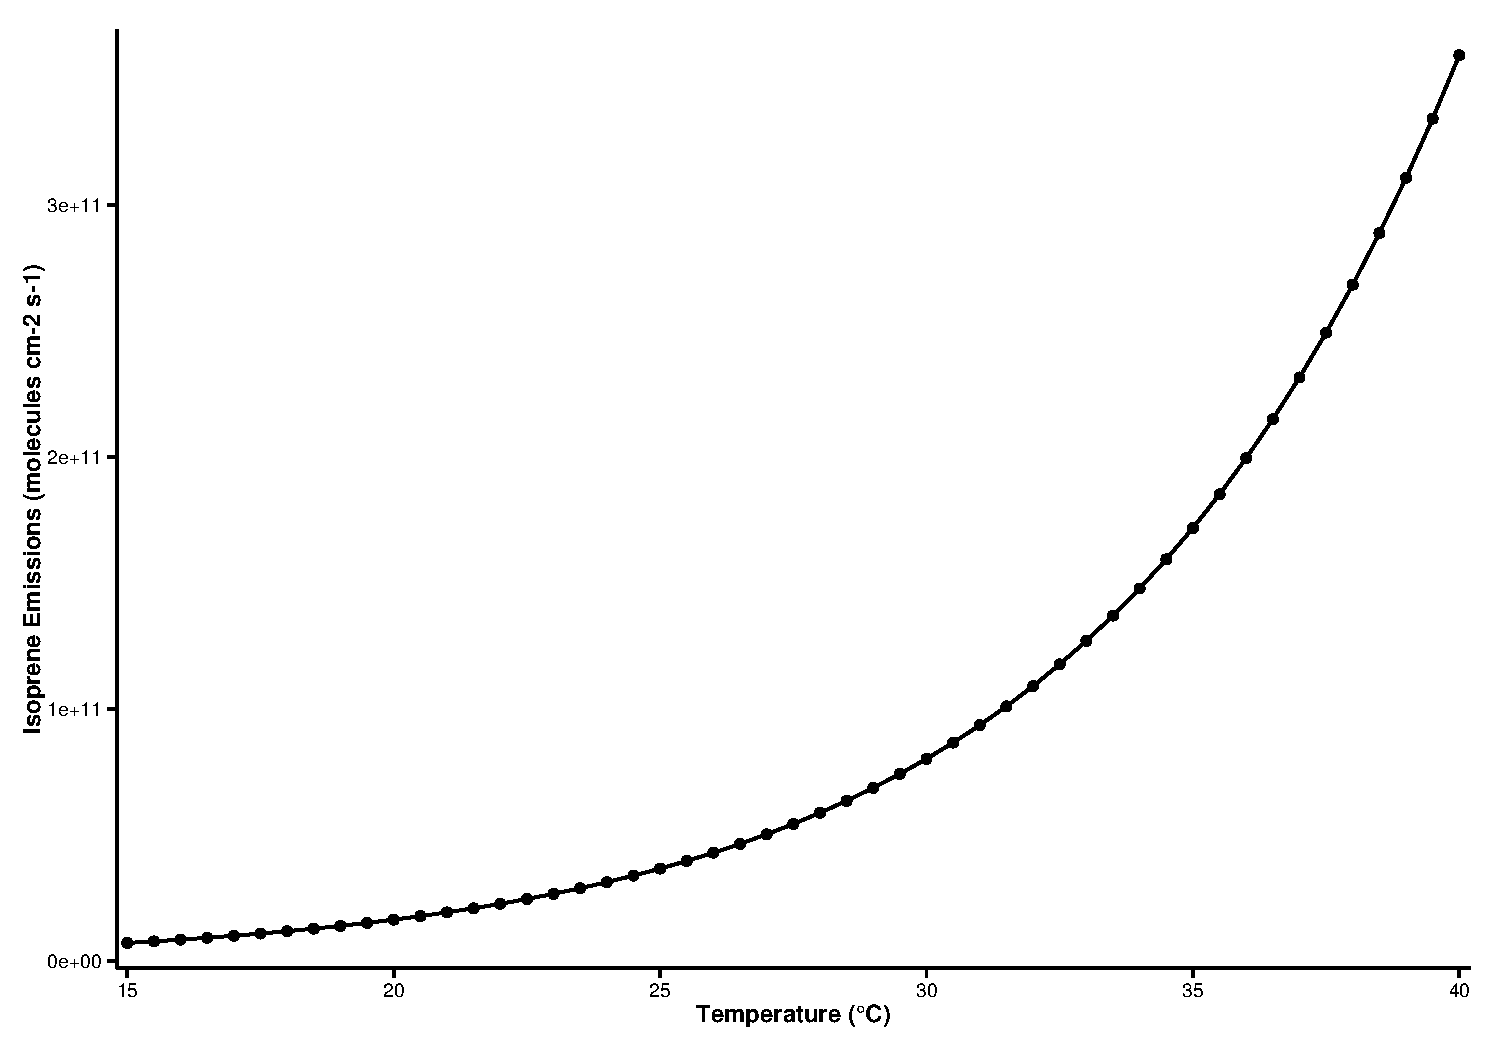
\includegraphics[width=\textwidth]{img/isoprene_emissions}
\end{figure}
Temperature-dependent emissions of isoprene were estimated using the MEGAN2.1 model for calculating the emissions of VOC from vegetation \citep{Guenther:2012}.
Emissions from plants are dependent on variables including temperature, radiation and age but for the purpose of our study we are only interested in the effects of temperature, hence all variables except temprature were held constant.

The MEGAN2.1 parameters were chosen to give similar isoprene mixing ratios at $20$~\degree C to the temperature-independent emissions, enabling an adequate comparison of the effects of increased isoprene emissions from the temperature-independent case.
The estimated emissions of isoprene with MEGAN2.1 using these assumptions, are illustrated in Fig.~\ref{f:isoprene_emissions} and show the expected exponential increase in emissions with temperature \citep{Guenther:2006}.

To verify whether our inputs to calculating isoprene emissions using MEGAN2.1, we compare the simulated isoprene mixing ratios to those measured from over the urban area of Essen, Germany \citep{Wagner:2014}.
At $20$~\degree C, the estimated emissions of isoprene lead to $0.07$~ppbv of isoprene in our model while at $30$~\degree C, the increased emissions of isoprene using MEGAN2.1 estimations lead to $0.35$~ppbv of isoprene in the model.
In the measurement campaign over Essen, $0.1$~ppbv of isoprene were measured at temperatures of $20$~\degree C and $0.3$~ppbv of isoprene were measured at $30$~\degree C.
This comparison indicates that the values chosen for calculating the temperature-dependent emissions of isoprene with MEGAN2.1 lead to reasonable values of isoprene mixing ratios.
